\documentclass[fontset=windows]{article}
\usepackage[]{ctex}
\usepackage[left=1.25in,right=1.25in,top=1in,bottom=1in]{geometry}
\usepackage{float}
\usepackage{graphicx} % Required for the inclusion of images
\usepackage{natbib} % Required to change bibliography style to APA
\usepackage{amsmath} % Required for some math elements 
\usepackage{fontspec}
\usepackage{graphicx}
\usepackage{booktabs}
\usepackage{subfig}
\usepackage[usenames]{xcolor}
\newfontfamily\monaco{Monaco}
\usepackage{listings}
\lstset{ %
    language=C++,                % the language of the code
    basicstyle=\small\monaco,           % the size of the fonts that are used for the code
    numbers=left,                   % where to put the line-numbers
    numberstyle=\tiny\color{gray},  % the style that is used for the line-numbers
    stepnumber=1,                   % the step between two line-numbers. If it's 1, each line 
                                    % will be numbered
    numbersep=5pt,                  % how far the line-numbers are from the code
    backgroundcolor=\color{white},      % choose the background color. You must add \usepackage{color}
    showspaces=false,               % show spaces adding particular underscores
    showstringspaces=false,         % underline spaces within strings
    showtabs=false,                 % show tabs within strings adding particular underscores
    frame=single,                   % adds a frame around the code
    rulecolor=\color{black},        % if not set, the frame-color may be changed on line-breaks within not-black text (e.g. commens (green here))
    tabsize=2,                      % sets default tabsize to 2 spaces
    captionpos=b,                   % sets the caption-position to bottom
    breaklines=true,                % sets automatic line breaking
    breakatwhitespace=false,        % sets if automatic breaks should only happen at whitespace
    title=\lstname,                 % show the filename of files included with \lstinputlisting;
                                    % also try caption instead of title
    keywordstyle=\color{blue},          % keyword style
    commentstyle=\color[RGB]{0,96,96},       % comment style
    stringstyle=\color[RGB]{96,0,96},         % string literal style
    escapeinside={\%*}{*)},            % if you want to add LaTeX within your code
    % morekeywords={*,...},              % if you want to add more keywords to the set
}

\title{LSM Tree实验报告}
\author{魏新鹏 519021910888}
\date{6月6日 2021年}

\usepackage{natbib}
\usepackage{graphicx}
\usepackage{enumitem}
\begin{document}

\maketitle

\section{背景介绍}
LSM Tree(Log-structured merge tree)是一种高性能的存储数据结构。传统关系型数据库使用B+ tree或一些变体作为存储结构,能高效进行查找。但保存在磁盘中时它有一个明显的缺陷,那就是逻辑上相离很近的数据物理上可能相隔很远,这就可能造成大量的磁盘随机读写。随机读写比顺序读写慢很多,为了提升IO性能,我们需要一种能将随机操作变为顺序操作的机制。LSM树能让我们进行顺序写磁盘,从而大幅提升写操作,作为代价的是牺牲了一些读性能。目前许多主流数据库,如Google的levelDB,FaceBook的RocksDB以及Apache的HBase的底层实现都采用了这种数据结构。

\begin{figure}[H]
\centering
\begin{minipage}[ht]{0.4\linewidth}   
    \centering   
    
\includegraphics[width=0.8\textwidth]{img/levelDB.jpg}
    \caption{levelDB}
    \label{fig:levelDB}
\end{minipage}
\begin{minipage}[ht]{0.4\linewidth} % 如果一行放2个图,用0.5,如果3个图,用0.33  
    \centering
    
\includegraphics[width=0.8\textwidth]{img/RocksDB.jpg}
    \caption{RocksDB}
    \label{fig:rocksdb}
\end{minipage} 
\begin{minipage}[ht]{0.4\linewidth} % 如果一行放2个图,用0.5,如果3个图,用0.33  
    \centering
    
\includegraphics[width=0.8\textwidth]{img/HBase.jpeg}
    \caption{Hbase}
    \label{fig:hbase}
\end{minipage}
\end{figure}

\section{挑战}
\subsection{设计}
这个project让我深深体会到了软件工程原理与实践那门课上沈老师讲的一句话:「一个项目要花70\%的时间在设计上,剩下30\%的时间用来编码。」回顾这个持续了整个后半学期的project,虽然项目文档中已经提供了详尽的说明,但仍有许多实现的具体细节需要斟酌,我也确实花了大量的时间在构思与设计上,整体结构也做了一次较大的更改。

我使用三个类来操作LSM Tree。
\begin{enumerate}
\item MemTable是内存中的存储,它包括一个跳表类,布隆过滤器数组和余量。
\begin{lstlisting}
class MemTable {
private:
    SkipList skList;
    bool * bloomFilter;
    int capacity;
};
\end{lstlisting}
\item Cache是SSTable中除了数据区外的部分,它包括Header,布隆过滤器数组和索引区。为了避免数据对齐造成的空隙,我没有将key与offset紧邻存储,而是使用了两个数组。
\begin{lstlisting}
class MemTable {
private:
    Header headerPart;
    bool * bloomFilter;
    uint64_t * keyArray;
    uint32_t * offsetArray;
};
\end{lstlisting}
\item SSTable是归并时的操作单元。它包括一个指向其对应的cache的指针和数据。
\begin{lstlisting}
class SSTable{
private:
    cache* SSTcache;
    char* SSTvalue;
};
\end{lstlisting}
\end{enumerate}

我面临的第一个问题便是如何将内存中的cache与硬盘中SSTable一一对应起来,其实这并不是一个复杂的问题,我最初的的处理方案是:因为SSTable的键值区间是不相交的,所以可以将文件名按照其从小到大的顺序排列从$0.sst$一直到$2^{n-1}.sst$,cache也按照这样顺序排列在\verb|std::list<cache*>|中。这种实现解决前两周的要求(即除compaction外的要求)都没有问题,但当我按照这种组织方式实现合并时,发现会涉及到大量文件的重命名与cache在\verb|std::list<cache*>|中位置的调整,随后我意识到维护这样的大小顺序并没有什么必要,在cache类中记录其对应的SSTable文件名即可。

第二个问题是合并的实现。其逻辑如图\ref{fig:compaction}所示。
\begin{figure}[h]
\centering
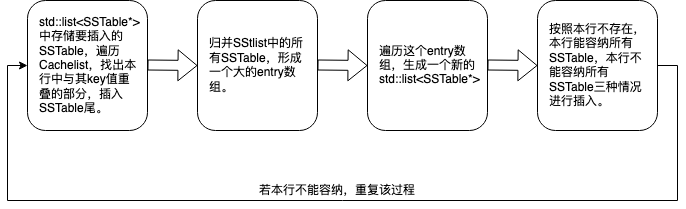
\includegraphics[width=1\textwidth]{img/campaction.png}
\caption{Compaction}
\label{fig:compaction}
\end{figure}

因为我的文件名采用int类型,大小从0开始增加,那么新的SSTable的文件名该如何取呢?如果是顺序插入,那么当前的size便是新插入SSTable的文件名,但如果一个文件被归并,那么它的文件名便空缺了出来,这里有两种方法解决这个问题,一是记录当前最大文件名(有点类似数据库的自增主键),但这会导致频繁读写的话文件名增加很快,甚至超出int表示范围。因此我为每一层维护一个\verb|std::vector<int> slot|表示这一层有多少个空缺的文件名,新插入的SSTable先从slot中找名字,再从size开始命名。

\subsection{Bug}
这里记录一下调试过程中解决的最大的Bug,这个Bug的解决也让我对C++ STL有了更深刻的理解。

我所碰到的问题是correctness和persistence有时能正常运行,有时却会出错,且出错的地方分布不一,这令我大为不解。这两个测试不是确定性的吗?为什么会有随机因素。我反复运行这两个测试文件,定位了几个高频出错点,然后在这几个高频出错点逐行调试。发现问题出在对\verb|std::list<cache*>|的删除。我是这么删除的:
\begin{lstlisting}
for(auto p = cacheList[line] -> begin(); p != cacheList[line] -> end(); p++){
    delete *p;
    cacheList[Line] -> erase(p);
}
\end{lstlisting}

这里的问题在于删除迭代器后再对迭代器做加一操作,这会导致不确定的行为。正确的做法应该如下。
\begin{lstlisting}
for(auto p = cacheList[line] -> begin(); p != cacheList[line] -> end();){
    delete *p;
    p = cacheList[Line] -> erase(p);
}
\end{lstlisting}

\section{测试}
\subsection{性能测试}
\subsubsection{预期结果}
\begin{description}
\item[Get] 内存中查找:跳表查找操作的时间复杂度为$O(\log n)$。硬盘中查找:先在cache中查找,因为每个cache都有bloomfilter,所以可以认为仅需$O(1)$即可判断是否在该SSTable中,判定存在后使用二分查找找到offset,时间复杂度也为$O(\log n)$。因此可以认为Get操作的时间复杂度是$O(\log n)$其中n为平均每个SSTable所容纳的键值对个数。但实际上硬盘读写需要大量时间,因此对于访问硬盘的Get操作,硬盘读写应占到了主要时间。
\item[Put] 不发生归并:不发生归并时仅在跳表中插入该键值对,先搜索跳表,查找该元素,这一步需要$O(\log n)$的时间,然后执行插入,因为跳表每一元素期望的塔高为2,因此可以在常数时间内完成插入。发生归并:具体的时间花费与数据的区间,硬盘中已经存在的数据分布情况有关。但无论如何,这一步都要花费相当多的时间。
\item[Delete] 先执行Get操作,如果找到再执行Put操作插入一条\verb|"~Delete~"|,因此其期望的时间复杂度应为Get与Put的和,但实际上因为插入的字符仅占8个字符,发生归并的概率不高,因此其实际时间复杂度应小于Get与Put复杂度的和。
\end{description}
\subsubsection{测试环境}
\begin{description}
\item[机型] MacBook Pro (13-inch, 2020, Four Thunderbolt 3 ports)
\item[处理器] 2 GHz 四核Intel Core i5
\item[内存] 32 GB 3733 MHz LPDDR4X
\item[SSD] APPLE SSD AP0512N 8.0 GT/s
\item[机械硬盘] My Passport 1TB Western Digital Technologies, Inc
\end{description}
\subsubsection{延迟测试}
我使用了两块硬盘进行了测试,一块是本机自带的固态硬盘,一块是外接机械硬盘。本机的雷电3端口可以提供高达40GB/s的传输速度,所以仅需考虑硬盘的读写速度差异。

我也使用了两种数据集进行了测试,随机数据与顺序数据。随机数据集为一个每个字符串长度为0到30000间随机值的字符串序列。顺序数据集为一个字符串长度单调递增的字符串序列,为了尽量保证插入的数据量与随机数据集接近,这个序列字符串长度的期望为15000。每次测试都会按照put,get,delete的顺序进行,即先执行n次put操作,再执行n次get操作,最后执行n次delete操作,分别统计三者的时间。为了减少偶然误差,每组都进行了三次实验,取平均值作为最终的结果。
\begin{enumerate}
\item 随机数据延迟测试。
\begin{figure}[H]
   \begin{minipage}[t]{0.5\linewidth}   
     \centering   
     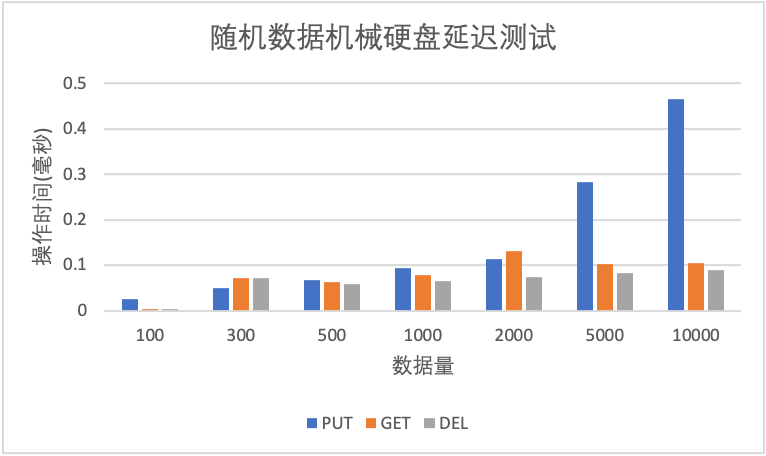
\includegraphics[width=0.9\textwidth]{img/random_latency_three.png}   
     \caption{机械硬盘各操作延时}   
     \label{fig:r_l_t}
   \end{minipage}
   \begin{minipage}[t]{0.5\linewidth} % 如果一行放2个图,用0.5,如果3个图,用0.33  
     \centering
     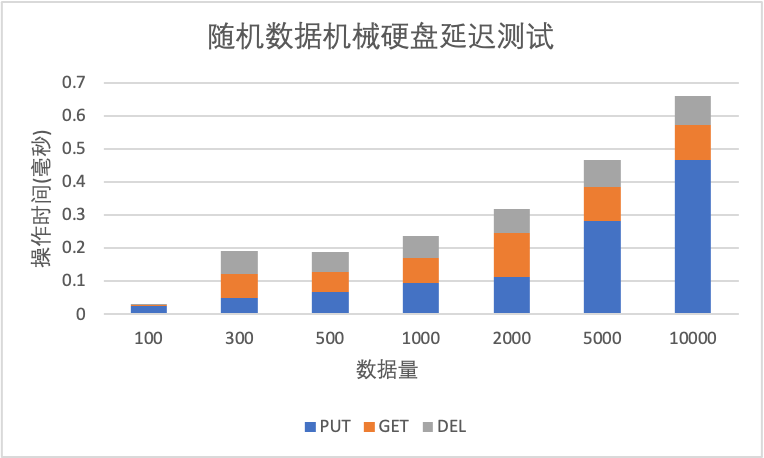
\includegraphics[width=0.9\textwidth]{img/random_latency_one.png}
     \caption{机械硬盘各操作延时占比}
     \label{fig:r_l_o}
    \end{minipage} 
\end{figure}
\begin{figure}[H]
   \begin{minipage}[t]{0.5\linewidth}   
     \centering   
     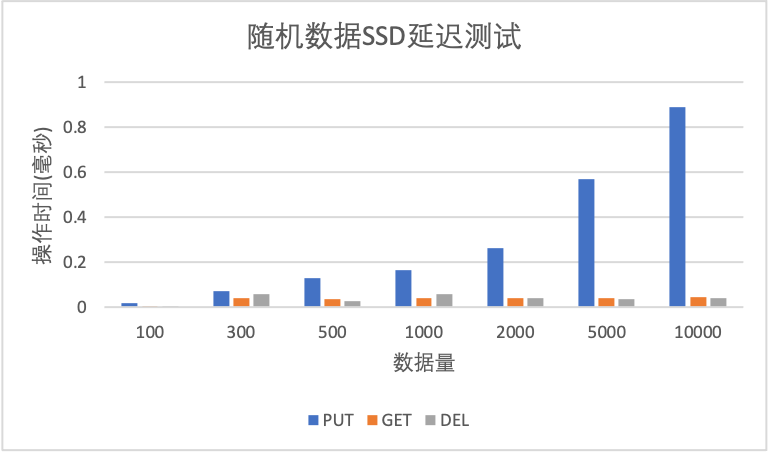
\includegraphics[width=0.9\textwidth]{img/random_SSD_latency_three.png}   
     \caption{SSD各操作延时}   
     \label{fig:r_S_l_t}
   \end{minipage}
   \begin{minipage}[t]{0.5\linewidth} % 如果一行放2个图,用0.5,如果3个图,用0.33  
     \centering
     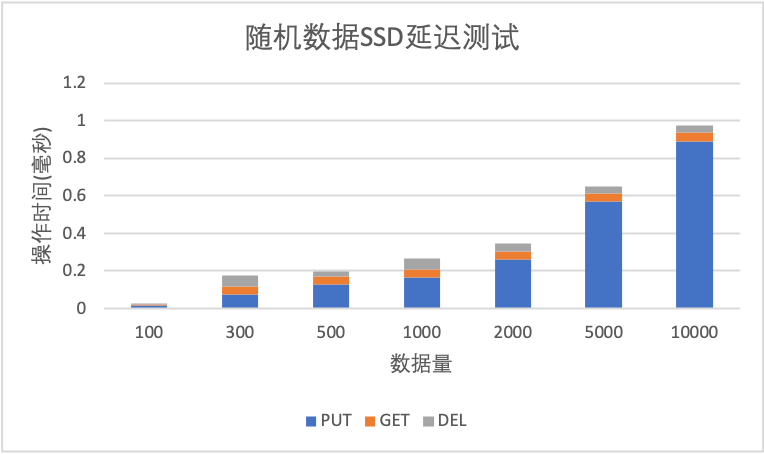
\includegraphics[width=0.9\textwidth]{img/random_SSD_latency_one.png}
     \caption{SSD各操作延时占比}
     \label{fig:r_S_l_o}
    \end{minipage} 
\end{figure}

通过图表可以看出对于机械硬盘,在数据量小时(2000以内,最多发生1至2次归并)三种操作耗时相近,且都随数据量的增加逐渐变大,这很好理解,数据量增加,插入操作会更多的写入硬盘,而读取与删除操作则更多的从硬盘中读取数据。对于机械硬盘,删除的耗时甚至小于读取,这令我有一丝疑惑,因为删除操作会先调用一次读取操作,通过查看具体的三组数据,我发现第一次实验的读取时间往往较大,拉高了平均值,而且通过数据量为100的测试我们可以发现,内存读取相比硬盘读取,时间几乎可以忽略,而删除操作插入的字符串很短,几乎不发生硬盘读写,因此在数据量较大时,删除操作的插入部分可以忽略。当数据量大时,因为要多次归并,插入操作的耗时明显增加,占比也随之增大。

对于SSD,总体趋势与机械硬盘相同,但是SSD插入操作的时间明显多余另外两个操作,与机械硬盘相比达到了同数据量机械硬盘插入操作的两倍。但读取与删除操只有机械硬盘耗时的50\%。SSD在插入操作上耗时较大可以进一步研究。
\item 顺序数据延迟测试。
\begin{figure}[H]
\begin{minipage}[t]{0.5\linewidth}   
    \centering   
    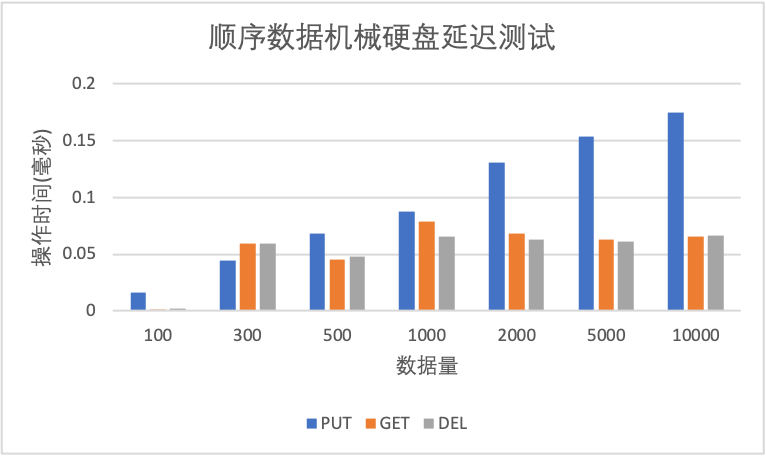
\includegraphics[width=0.9\textwidth]{img/sequential_latency_three.png}   
    \caption{机械硬盘各操作延时}   
    \label{fig:s_l_t}
\end{minipage}
\begin{minipage}[t]{0.5\linewidth} % 如果一行放2个图,用0.5,如果3个图,用0.33  
    \centering
    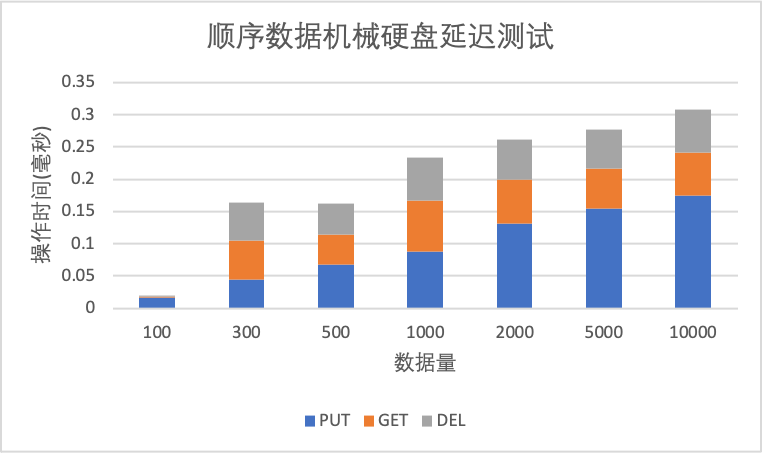
\includegraphics[width=0.9\textwidth]{img/sequential_latency_one.png}
    \caption{机械硬盘各操作延时占比}
    \label{fig:s_l_o}
\end{minipage} 
\end{figure}
\begin{figure}[H]
   \begin{minipage}[t]{0.5\linewidth}   
     \centering   
     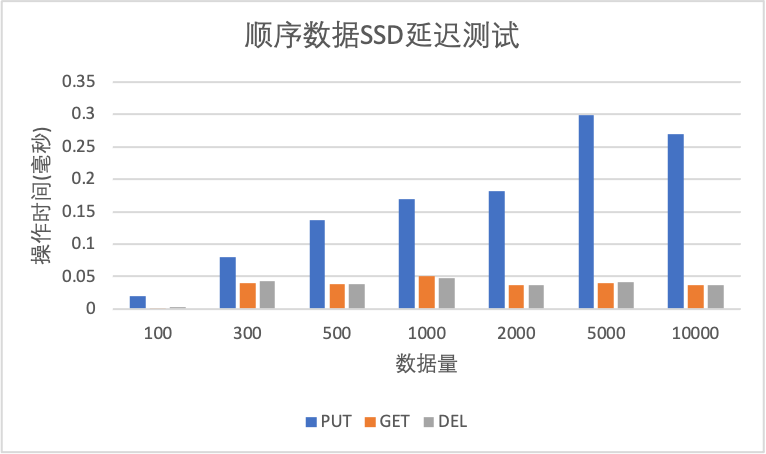
\includegraphics[width=0.9\textwidth]{img/sequential_SSD_latency_three.png}   
     \caption{SSD各操作延时}   
     \label{fig:s_S_l_t}
   \end{minipage}
   \begin{minipage}[t]{0.5\linewidth} % 如果一行放2个图,用0.5,如果3个图,用0.33  
     \centering
     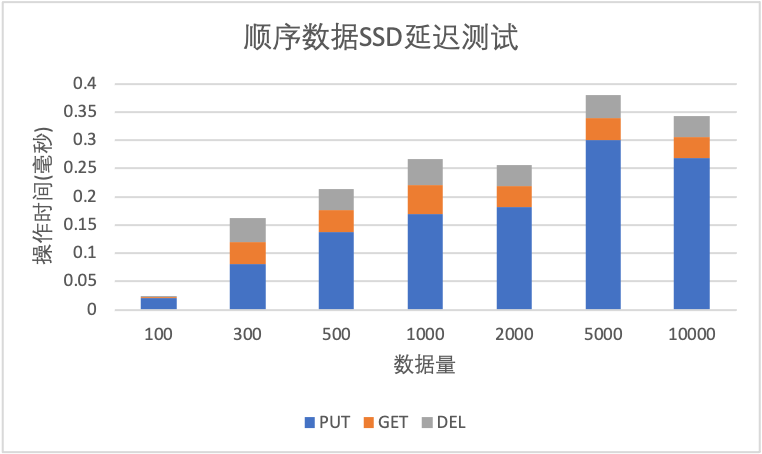
\includegraphics[width=0.9\textwidth]{img/sequential_SSD_latency_one.png}
     \caption{SSD各操作延时占比}
     \label{fig:s_S_l_o}
    \end{minipage}
\end{figure}
通过图表可以看出总体趋势依然是各操作的时间随着数据量的增大而增加,且SSD相比机械硬盘,插入慢了一倍,读取与删除快了一倍,但与随机数据不同的是大数据量时插入操作的时间减少为了原先的40\%\textasciitilde 50\%。这是因为顺序数据的键值区间与下一行并不重叠,因此归并时无需读入下一行的数据。
\end{enumerate}
\subsubsection{吞吐量测试}
操作的吞吐为其延迟的倒数,因此我们可以直接使用延迟测试中的实验数据。
\begin{figure}[H]
\begin{minipage}[t]{0.5\linewidth}   
    \centering   
    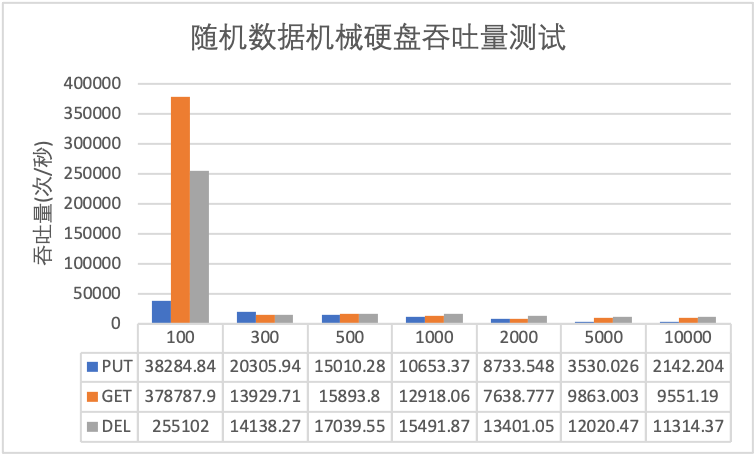
\includegraphics[width=0.9\textwidth]{img/random_throughput.png}   
    \caption{机械硬盘随机数据吞吐}   
    \label{fig:r_t}
\end{minipage}
\begin{minipage}[t]{0.5\linewidth} % 如果一行放2个图,用0.5,如果3个图,用0.33  
    \centering
    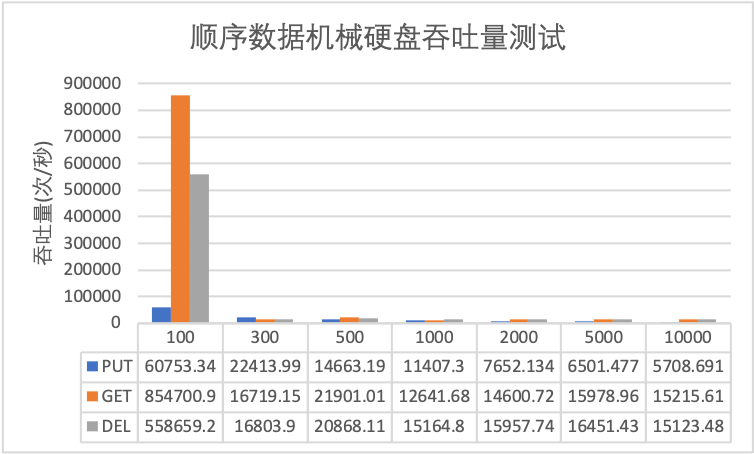
\includegraphics[width=0.9\textwidth]{img/sequential_throughtput.png}
    \caption{机械硬盘顺序数据吞吐}
    \label{fig:s_t}
\end{minipage} 
\end{figure}
\begin{figure}[H]
   \begin{minipage}[t]{0.5\linewidth} % 如果一行放2个图,用0.5,如果3个图,用0.33  
     \centering
     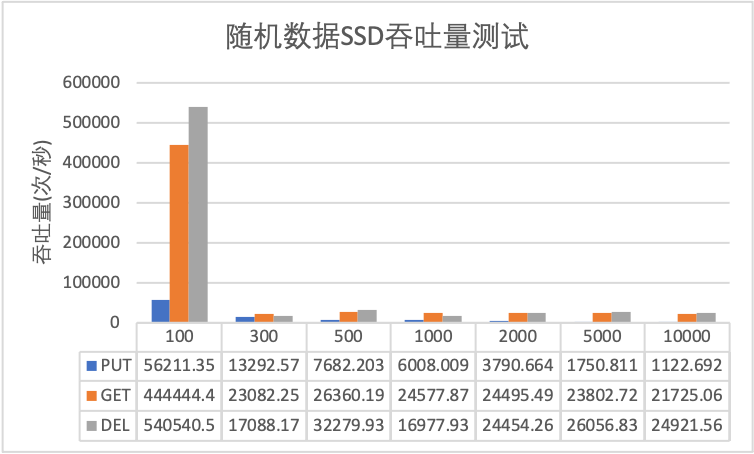
\includegraphics[width=0.9\textwidth]{img/random_SSD_throughput.png}
     \caption{SSD随机数据吞吐}
     \label{fig:r_S_t}
    \end{minipage}
    \begin{minipage}[t]{0.5\linewidth}   
     \centering   
     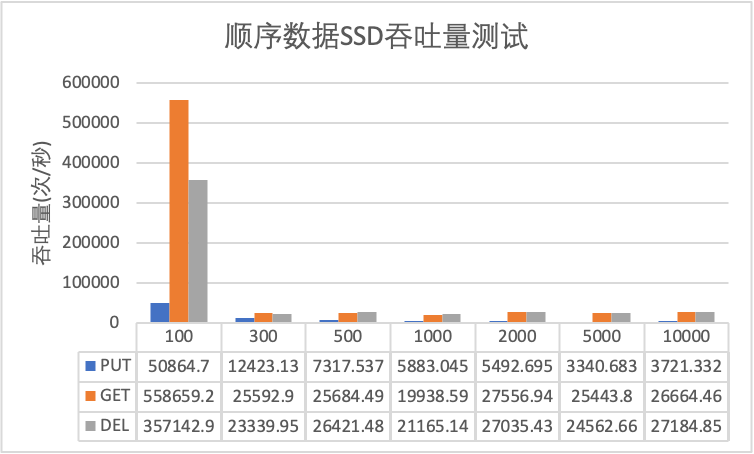
\includegraphics[width=0.9\textwidth]{img/sequential_SSD_throughput.png}   
     \caption{SSD顺序数据吞吐}   
     \label{fig:s_S_t}
   \end{minipage}
\end{figure}


\subsubsection{索引缓存与Bloom Filter的效果测试}
\begin{enumerate}
    \item 内存中没有缓存SSTable的任何信息,从磁盘中访问SSTable的索引,在找到offset之后读取数据。
    \item 内存中只缓存了SSTable的索引信息,通过二分查找从SSTable的索引中找到offset,并在磁盘中读取对应的值。
    \item 内存中缓存SSTable的Bloom Filter和索引,先通过Bloom Filter判断一个键值是否可能在一个SSTable中,如果存在再利用二分查找,否则直接查看下一个SSTable的索引。
\end{enumerate}
\begin{figure}[ht]
\centering
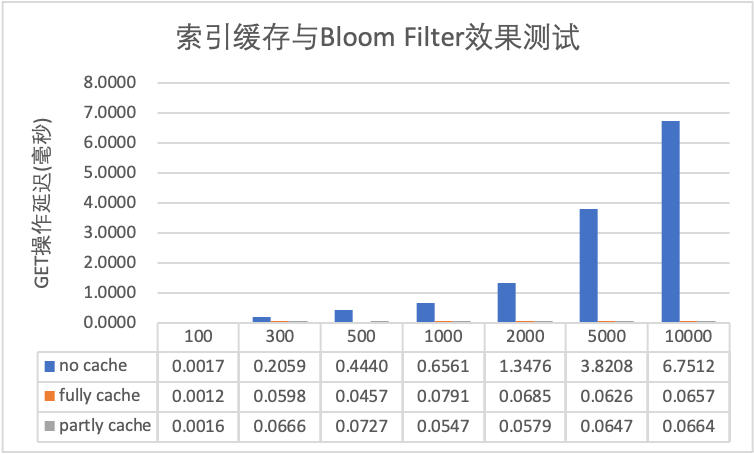
\includegraphics[width=0.8\textwidth]{img/bloomFilter_cache_test.png}
\caption{bloomFilter and cache Test}
\label{fig:b_c_test}
\end{figure}

从图像可以看出,内存中缓存索引信息能显著提升查询的效率,bloomFilter则能进一步提升查询效率。
\subsubsection{Compaction的影响}
连续插入400000条数据,每条数据为\verb|std::string(500,'s')|,统计每插入100条的时间。理论上每插入约4000条数据会将内存中的数据写入SSTable,每插入三个SSTable会发生一次归并。实验并绘制图像如下图所示。
\begin{figure}[ht]
\centering
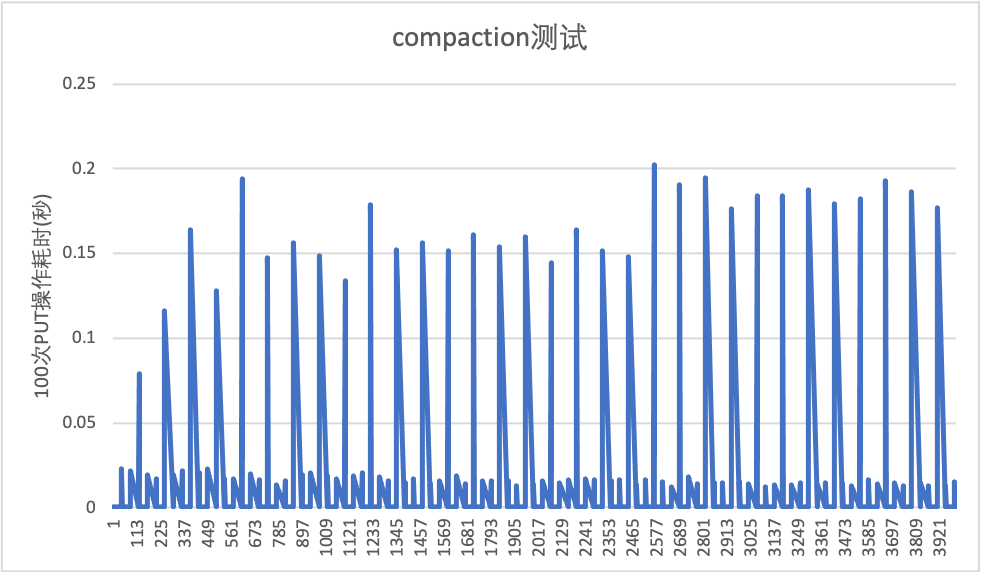
\includegraphics[width=0.8\textwidth]{img/compaction_test.png}
\caption{Compaction Influence}
\label{fig:compaction_test}
\end{figure}

观察图像发现每隔约40组数据会有一个小峰,每隔约120组数据会有一个高峰。这与理论是相符的。
\section{收获}
本学期虽有很多很多的lab、project,但这个project给我留下了非常深刻的印象。一开始陷入错误的设计之中,写了非常复杂的归并操作,一度难以进行,后来修改了设计,豁然开朗,这让我深深体会到了设计的重要性,也给之后的项目带来了一些启示:要想的深入一些,想想具体的代码该怎么写,而不只是脑海中大致觉得这么写就差不多了。正所谓「Talk is cheap,Show me the code.」

还有模块化,其实我不是一开始就分好了一个个类与函数的,我的PUT操作一开始有300多行,在逐步完善及实现其他功能的过程中,我发现了重复的部分,发现了共同使用的数据结构,于是把他们封装为函数,类。

这个project的Debug过程也十分痛苦,因为它涉及到大量文件操作,程序执行时间较长,再加上错误不是每次都会发生,导致调试变得很困难。而最后问题的解决基本都是靠着大量打印信息,逐行调试,添加观察变量再逐行分析。

最后,纸上得来终觉浅,绝知此事要躬行。没有什么能比自己动手实现一遍更好的掌握一个数据结构了。感谢老师与助教设计这么好的project。
\end{document}